\documentclass[11pt,a4paper]{article}

\usepackage[utf8]{inputenc}
\usepackage[english]{babel}
\usepackage{amsmath}
\usepackage{amsfonts}
\usepackage{amssymb}
\usepackage{graphicx}
\usepackage{hyperref}
\usepackage{pdflscape}
\usepackage{times}
\usepackage{geometry}
\usepackage{scalerel}

\author{António Carvalho}

\geometry{
	a4paper, 
	total = {6in, 8in},
	left = 20mm,
	right = 20mm,	
	textheight = 700pt
}


\begin{document}
\renewcommand{\baselinestretch}{1.2}

%\thispagestyle{empty}


\begin{figure}[ht!]
	\vspace*{-2.9cm}
	\centering
	\scalebox{0.5}{
\includegraphics{Figures/Logo_ISEL}}
\end{figure}

\vspace*{-1.5cm}

\begin{center}
Licenciatura em Engenharia Informática e de Computadores \\
Projeto e Seminário - Semestre de verão 2022/2023 \\
\end{center}

\begin{center}
{\large \textbf {Project Proposal}}
\end{center}	

\smallskip

\renewcommand{\arraystretch}{1.2}
 	\begin{center}
		\begin{tabular}{ p{3 cm} p{2 cm} p{3.6 cm}  }
			\multicolumn {3}{c}{ \large{\textbf{Author}}} \\
			\hline
			 António Carvalho & 48347 &  a48347@alunos.isel.pt \\
		\end{tabular}
	\end{center}

\smallskip


\renewcommand{\arraystretch}{1.2}
	\begin{center}
		\begin{tabular}{ p{3 cm} p{3.6 cm}  p{2cm} }
			\multicolumn{3}{c}{\large{\textbf{Advisor}}} \\
			\hline
			 Nuno Leite  &  nuno.leite@isel.pt & ISEL \\
		\end{tabular}
	\end{center}

\vspace{5mm}

\section{Title}

\textbf{PostChat} - "Bring Back Postcards" - Smart Chat service using handwritten postcards.
	

\section {Introduction and State of the Art}
	Keeping in touch with your relatives might be a bit of a hassle, specially for those that have a hard time with new technologies. \par
	With that in mind our application focuses on keeping things simple for people of age, while still appealing to everyone.
	Our goal is simple, to bring back postcards, adapting it to the new digital era.\par
	With PostChat you can choose your postcard template and start writing on the touchscreen.\par
	Our application offers accessibility features like Optical Character Recognition \cite{IBM2023}, in order to transcript handwritten text to computer alphanumeric, and Text-To-Speech \cite{Oracle2023}.\par
	Apps and services like Postcard App \cite{Ltd2023} have a different approach. Unlike our project these apps are paid for to sent physical postcards.
	Our app is completely free and aims to send digital postcards to wherever in the globe as a beautiful and modern form to connect to your relatives.

\section{Objectives}
	\begin{itemize}
		\item Develop and research an OCR model using neural networks in order to extract the postcard content.
		\item Develop a web API to support our application.
		\item Create a frontend application for Android using Jetpack Compose framework.
		\item Research and implement TTS on the application.
	\end{itemize}

\section{Justification}
	This project will allow us to be prepared for the new AI world and to extend and improve all the knowledge gained until this point. \par
	
	
	 
\section{Scope}
	This application's scope is quite broad as any individual can access it for personal use.\par
	Because PostChat uses the internet to send messages, it can be used for international communication without incurring international text or call charges.

\section{Approach and Delivery}
	\subsection{Approach}
	Our approach can be separated in 4 independent components. 
	\begin{itemize}
		\item \textbf{AI} - Train a OCR \cite{IBM2023} model using Python language \cite{Python2023} and TensorFlow with Keras \cite{Tensorflow2023} framework. 
		\begin{itemize}
			\item The idea is to create a neural network to detect handwritten text present in postcards sent by users, to do so we will train our model using the IAM \cite{IAM2023} dataset. 
		\end{itemize}
		\item \textbf{Storage} - Data will be encrypted and stored in a PostgreSQL \cite{Postgres2023} database.
		\begin{itemize}
			\item The only permanent data stored is user's log in information. All data meant to be sent by one user to another (postcards and generated transcript text from OCR) is stored temporally until sent by the server. 
		\end{itemize}
		\item \textbf{WEB API} - A web API written in Kotlin \cite{Kotlin2023} using Spring framework \cite{Spring2023}.
		\begin{itemize}
			\item In order to make this project work we will make a reactive HTTP/S API.
			\item ProcessBuilder is used to make the connection between the AI code in Python and the JVM.
		\end{itemize}
		\item \textbf{Frontend} - Android application made using Android Jetpack Compose \cite{Compose2023}.
		\begin{itemize}
			\item Users will choose between various different postcard templates.  
			\item When in the application users will be asked permission to access their contacts in order to find all the users that have used the service.
			\item Will have to work with android notifications.
			\item Has to support different theme colors.
			\item Has to support landscape and portrait mode.
			\item Will keep a connection open in the background to the API.
		\end{itemize}
	\end{itemize}

	\vspace{20mm}
			\begin{figure}[ht!]
				\vspace*{-2.30cm}
				\centering
				\scalebox{0.39}{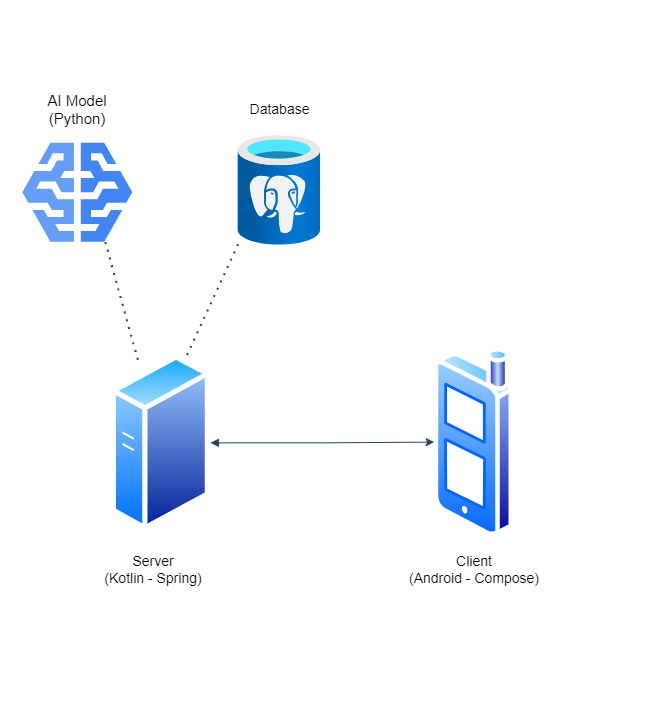
\includegraphics{Figures/Sketch.png}}
				\caption{Project Architecture.}
			\end{figure}
	\subsection{Delivery}
	At the end of this project it's expected to deliver a fully functional, easy to use and feature rich android application (same style as WhatsApp), as well as have a working
	AI model based on neural networks, that later might be exposed to the public as a stand-alone service.

\section{Restrictions and Premises}
	\begin{itemize}
		\item All new technologies used like AI, ProcessBuilder, and TTS will need research. 
		\item All functionalities need to be hand-to-hand with unit tests.
		\item Deadlines will need to be met with no exception.	
	\end{itemize}

\section{Resources}
	This project will be build using mainly open-source tools and frameworks. 
	An Android tablet might be needed for easy of work with the drawing portion of the application. 

\section{Risks}
	Managing time will be crucial in this project, planing alternatives for each and every new technical field is part of the success.
	Knowing to adopt and mold our goals and expectations is important in order to deliver a working project in case any problem occurs during the project's lifecycle. 
\section{Project Structure}
	This project will be made by António Carvalho and advised by Nuno Leite, teacher at ISEL. 
\section{Project Milestones}
	\begin{itemize}
		\item Project Proposal : March 20th 2023
		\item Progress Presentation : April 24th 2023
		\item Beta version : June 5th 2023
		\item Final version : July 10th 2023
	\end{itemize}


\newgeometry{left=5mm, right=5mm, top=0.5cm}

\section{Project Planing}
		\begin{figure}[htp]
		\centering
		\vstretch{.7}{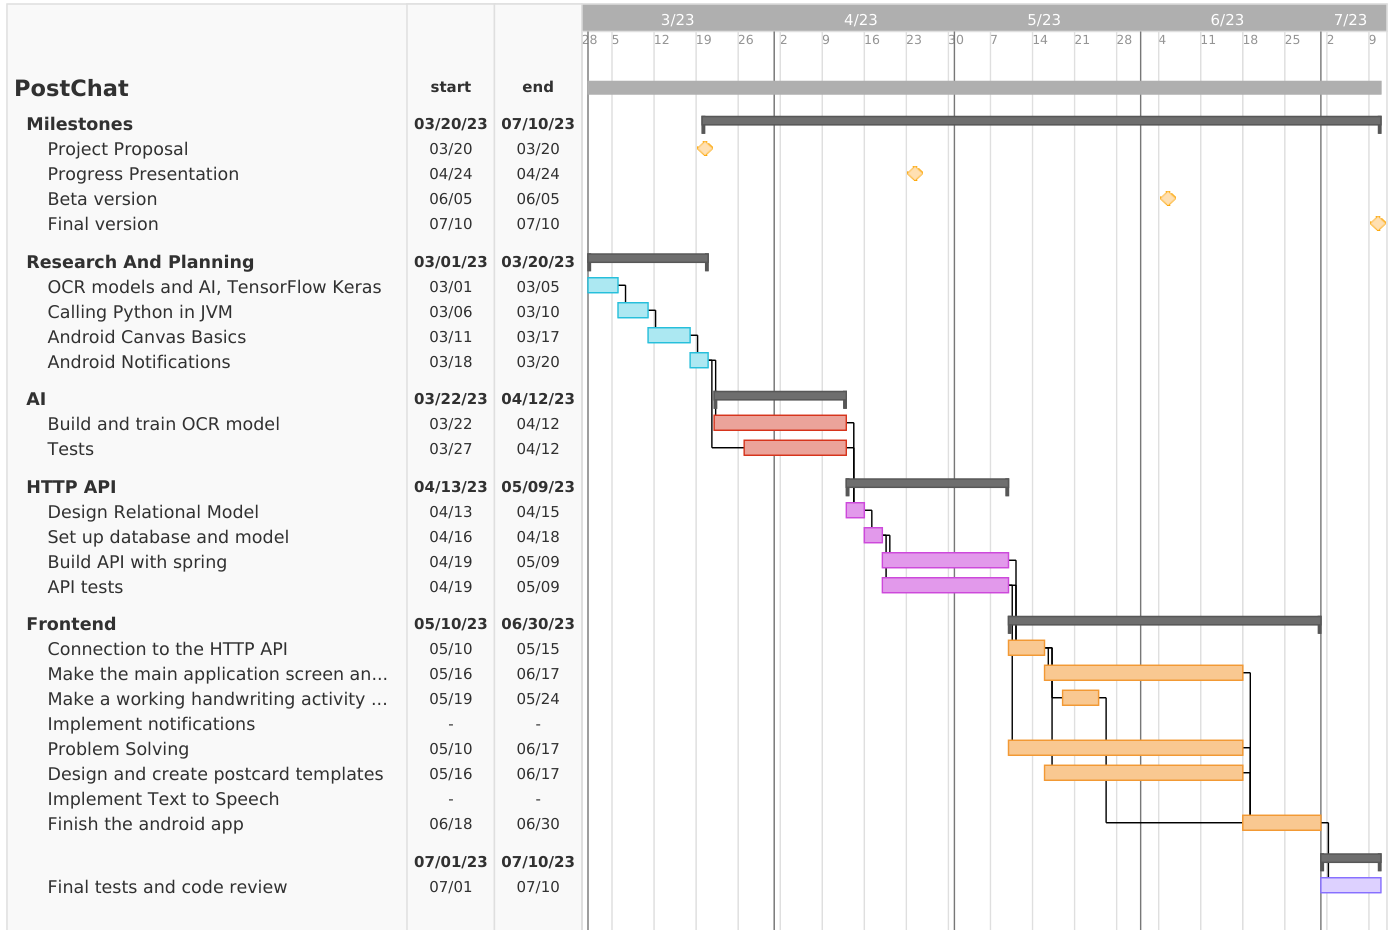
\includegraphics[width=20cm]{Figures/Gantt.png}}
		\caption{Gantt chart.}
		\end{figure}

\vspace*{-10mm}
%% APA style
\bibliographystyle{elsarticle-num}
\bibliography{References/References} % References.bib file
%

	
\end{document}